\chapter{Standby} \label{ch:standby}

Entanglement is at the heart of many quantum problems and applications~\cite{horodecki2009quantum}.   
Even though it has been studied for a long time now, entanglement is still a mysterious resource and understanding its power and limitations is an interesting area of research.  
Given a quantum state, determining whether it is entangled or separable (i.e., not entangled) is called the \emph{separability problem}.  
More precisely, for a density operator acting on the bipartite space $\A \otimes \B$, we wish to decide whether it belongs to the set of separable states, defined as 
\begin{equation} 
\SepD(\A: \B) = \mathrm{conv} \; \{ \rho \otimes \sigma \} 
\label{eq:ch2_SEP-SepIntro}
\end{equation} 
where $\mathrm{conv}$ denotes the convex hull (the set of all convex combinations), $\rho$ ranges over density operators on $\A$, and $\sigma$ ranges over density operators on $\B$. 
This problem is known to be NP-hard in general~\cite{gurvits2004classical,gharibian2010strong}. 
If $\dim(\A) \cdot \dim(\B) \leq 6$, then it turns out that this problem has a finite-sized semidefinite programming formulation~\cite{horodecki1996necessary} while for all other cases, it was shown that no finite-sized semidefinite program exists~\cite{fawzi2021set}. 

In this work, we also look at the set of separable \emph{operators} which is  defined as  
\begin{equation} 
\Sep(\A: \B) = \mathrm{conv} \; \{ X \otimes Y \} 
\label{eq:ch2_SEP-Sep}
\end{equation} 
where $X$ is a positive semidefinite operator acting on $\A$ and $Y$ is a positive semidefinite operator acting on $\B$. 
We note that $\Sep(\A: \B)$ and $\SepD(\A: \B)$ differ only in the fact that the latter has a unit trace constraint. 

A general linear optimization over the set of separable operators takes the form 
\begin{equation} \label{eq:ch2_SEP-Sep_opt_operator} 
\text{maximize } \Big\{ \inner{X}{C} : \Xi(X) = B, X \in \Sep(\A:\B) \Big\} 
\end{equation} 
where $C$ and $B$ are Hermitian matrices, $\Xi$ is a hermiticity-preserving linear map, and $\inner{A}{B}$ denotes the Hilbert-Schmidt inner product between two operators $A$ and $B$, which is defined as $\Tr(A^* B)$.  
While we consider the general problem above in this work, we often focus on the special case of linear optimization over the set of separable \emph{states} taking the form 
\begin{equation} \label{eq:ch2_SEP-Sep_opt} 
\text{maximize } \Big\{ \inner{\tau}{C} : \tau \in \SepD(\A:\B) \Big\}.  
\end{equation} 
Despite having a diverse array of applications~\cite{ioannou2007computational, brandao2011quasipolynomial, gharibian2013qma, chailloux2012complexity, hayden2013two, li2014quantum, consiglio2022variational, jeronimo2023power}, 
this problem is hard for two key reasons.   
For one, even if one were to exhibit a purported optimal solution, verifying its separability could be (NP) hard. 
Also, it suffers from the curse of dimensionality. 
In particular, when $\A$ and $\B$ represent $n$-qubit spaces, then $\tau \in \SepD$ has dimension $2^{2n}$ which renders many numerical computations infeasible. 

Quantum state discrimination is a central task in quantum information processing.
Quantum key distribution~\cite{ko2018advanced}, two-party cryptography~\cite{aharonov2000quantum, ambainis2001new, sikora2017simple}, the hidden subgroup problem~\cite{hayashi2008quantum}, and dimension witnessing~\cite{strubi2013measuring}, among many others, can all be formulated in terms of this problem, which can be described as the following two-party game.
Alice chooses a state from a fixed set of states and sends it to Bob who wishes to identify the state. 
Here we assume that both Alice and Bob know the set of states and the a priori probabilities before the game commences.

For Bob to determine his state perfectly, the necessary and sufficient condition is that the states in the set must be pairwise orthogonal.
However this need not be the case and, in such circumstances, Bob may wish to optimize some desired figure of merit, e.g., the average probability of correctly identifying the state.
Several other figures of merit exist depending on the desired application.
For example, Bob may wish to only guess when he knows he will be correct, called unambiguous state discrimination.
Each figure of merit could correspond to adopting a different strategy which would in turn lead to different behaviour.  
We discuss several variants in this work and refer the interested reader to the following reviews~\cite{chefles2000quantum, bergou200411, bergou2007quantum, barnett2009quantum, bergou2010discrimination}. 

Preparing and measuring quantum states are the two pillars of quantum computing. 
As an example, quantum state tomography is the task of identifying which quantum state a device is preparing given (many) samples~\cite{christandl2012reliable, torlai2018neural, gross2010quantum, qi2013quantum, ahmed2021quantum, mahler2013adaptive, schwemmer2015systematic}
which has been experimentally tested~\cite{cramer2010efficient, stricker2022experimental, rambach2021robust, rippe2008experimental, mallet2011quantum}. 
In other words, one wishes to find the best measurement(s) to perform in order to learn the state with the fewest number of samples. 

Another task central to quantum computing is the \emph{quantum state discrimination problem} where one is tasked with identifying which state they have been given \emph{from a fixed set of quantum states}. 
This is a naturally occurring setting which has been studied in the context of quantum algorithms~\cite{radhakrishnan2009random, hayashi2006quantum}, quantum cryptography~\cite{van2002unambiguous, cabello2000quantum, ambainis2001new, sikora2017simple}, quantum machine learning~\cite{sentis2016quantum, sentis2017exact}, among many others (see~\cite{Bae_2015} for a survey).  

The quantum state discrimination problem can be phrased as a game between Alice and Bob. 
Alice has a finite set of quantum states $\{ \rho_1, \ldots, \rho_n \}$ and a fixed probability distribution $(p_1, \ldots, p_n)$, both of which are known to Bob. 
Alice then samples $i$ with probability $p_i$ and prepares and sends $\rho_i$ to Bob. 
Bob wins the game if he correctly identifies the state by sending the correct index, $i$, back to Alice. 
This game is illustrated in Fig.~\ref{fig:ch4_PBM-fig1}.  
\begin{figure}[h] 
    \centering
    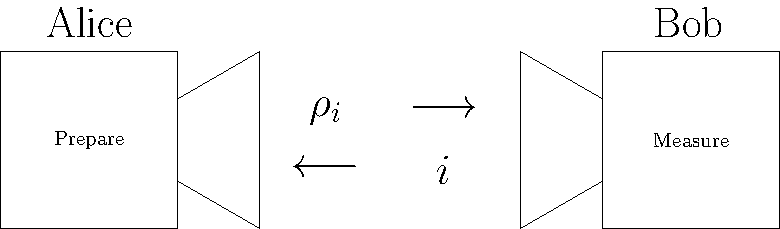
\includegraphics[scale=0.75]{figs/ch4_PBM/qsd_figure.pdf}
    \caption{Alice prepares $\rho_i \in \{ \rho_1, \ldots, \rho_n \}$ and sends it to Bob. 
    Bob wins the game if he correctly identifies the index $i$.}
    \label{fig:ch4_PBM-fig1}
\end{figure}

One can easily show that Bob can win this game perfectly if and only if the states have orthogonal supports, i.e., $\inner{\rho_i}{\rho_j} = 0$ for all $i \neq j$. 
When this is not the case, Bob may wish to maximize his probability of winning. 
Suppose he measures with the POVM $\{M_1, \ldots, M_n\}$ and on outcome $j$ he guesses the state was $\rho_j$. 
Then, given state $\rho_j$, he guesses ``I think the state is $\rho_i$'' with probability 
$\inner{M_i}{\rho_j}$.  
In this case, he wins the game with probability 
%\begin{equation} 
$\sum_{i=1}^n p_i \inner{M_i}{\rho_i}$.  
%\end{equation} 
If Bob wishes to maximize this probability, then he is tasked with finding the best POVM $\{M_1, \dots, M_n\}$, known as the \emph{minimum error} measurement, and we define the best probability for Bob as 
\begin{equation}
    \label{eq:ch4_PBM-P_best} 
    \Pbest = \text{max} \; \sum_{i=1}^n p_i \inner{M_i}{\rho_i}.
\end{equation} 

Given a problem instance, one can numerically solve for the best POVM using semidefinite programming~\cite{cvx}. 
Unfortunately, characterizing such POVMs is a difficult task known only to be possible in special cases, e.g., for $n=2$ the case of two states~\cite{helstrom1969quantum}, for $n$ arbitrary qubit states given with equal \emph{a priori} probabilities~\cite{deconinck2010qubit}, for geometrically uniform states~\cite{eldar2004optimal}, and mirror symmetric states~\cite{andersson2002minimum}.  
Therefore, it is important to find generic classes of measurements which have a simple form and \emph{approximate} $\Pbest$. 

%%%%%%%%%%%%%%%%%%%%%%%%%%%%%%%%%%%%%%%%%%%%%%%%%%%%%%%%%%%%%%%%%%%%%%%%%%%%%%%%%%%%%%%%%%%%%%%%%%%%%%%%%%%%%%%%%%%%%%%%%%%%%%%%%%%

\section{Quantum state exclusion} \label{sec:ch4_PBM-QSE}

The quantum state \emph{exclusion} problem is similar to quantum state discrimination except that Bob wishes to guess a state \emph{which was not sent}. 
For example, if Alice sends $\rho_1$ to Bob and Bob responds with ``Alice, you did not send $\rho_3$'' then he would win the game in that case. 
The work in \cite{bandyopadhyay2014conclusive} studies this task in detail and its relationship to the PBR game~\cite{pusey2012reality}. 
Quantum state exclusion is illustrated in Fig.~\ref{fig:ch4_PBM-fig2}.  
\begin{figure}[h] 
    \centering
    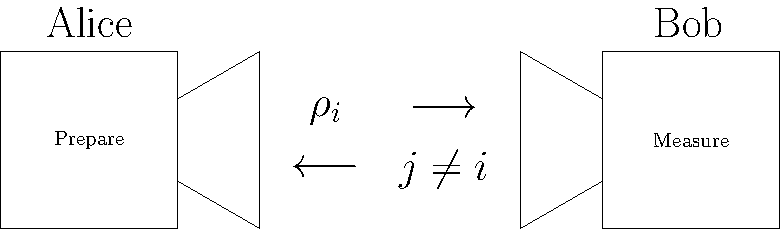
\includegraphics[scale=0.75]{figs/ch4_PBM/qse_figure.pdf}
    \caption{Alice prepares $\rho_i \in \{ \rho_1, \ldots, \rho_n \}$ and sends it to Bob. 
    Bob wins the game if he correctly \emph{excludes} an index $j \neq i$.}
    \label{fig:ch4_PBM-fig2}
\end{figure} 

Unlike quantum state discrimination, it is much more difficult to determine when Bob has a perfect strategy to perfectly win this game, i.e., when he can exclude a state without error. 
If this is the case, we say that the states are \emph{antidistinguishable} which has been the topic of recent research~\cite{havlivcek2020simple, russo2023inner, leifer2020noncontextuality, mishra2023optimal, uola2020all, johnston2023tight}. 

If Bob wishes to find the measurement which best excludes a state, he wishes to minimize the probability of making an incorrect guess.
More precisely, if Bob measures $\rho_i$ with the POVM $\{M_1, \ldots, M_N\}$, he makes an \emph{incorrect guess} with probability $\inner{M_i}{\rho_i}$.  
Thus, he wishes to \emph{minimize} 
%\begin{equation} 
$\sum_{i=1}^n p_i \inner{M_i}{\rho_i}$.  
%\end{equation} 

Notice that this is the exact opposite of what he wishes to do in the quantum state discrimination problem where he wants to maximize this quantity, see Eq.~\eqref{eq:ch4_PBM-P_best}. 
Thus, if Bob wants to exclude a state, his best measurement is also the \emph{worst} measurement for discrimination. 
Therefore, we define 
\begin{equation}
    \label{eq:ch4_PBM-P_worst}
    \Pworst = \text{min} \; \sum_{i=1}^k p_i \inner{M_i}{\rho_i}. 
\end{equation}

It is worth noting that the viewpoint of Bob trying to lose the quantum state discrimination game is interesting in its own right. 
Indeed, Bob cannot always lose this game with certainty, even if he wants to, and understanding when this is the case, and more generally, understanding the above quantity gives insights into the very nature of quantum information. 


The pretty good measurement (PGM), first discussed in~\cite{belavkin1975optimaldist, belavkin1975optimal, hughston1993complete}, is a way to approximate the best possible measurement. 
Sometimes PGM is optimal, some nice examples being for the hidden subgroup problem~\cite{bacon2005optimal, moore2005distinguishing}, for the quantum change point problem~\cite{sentis2016quantum}, and in port-based teleportation~\cite{leditzky2022optimality}.  
Generally speaking, for problems with a large amount of symmetry, the PGM seems to perform well. 

This brings us to the main question of this chapter:
\begin{center}
\textit{Is there an analogue of the pretty good measurement for approximating $\Pworst$?} 
\end{center}

We now review PGMs which helps us give an answer to the above question.

\amnote{Move this to the introduction}
Quantum state discrimination (refer~\cite{chefles1998quantum, barnett2009quantum,bae2015quantum, bergou2004discrimination} for reviews) provides the broader context for this problem. 
Here, a learner is presented with a quantum state drawn from a known ensemble, i.e., a collection of quantum states together with their \textit{a priori} probabilities, and the goal is to infer the identity of the given state. 
This is a fundamental task in quantum communication and cryptography, and the impossibility of perfect discrimination among non-orthogonal quantum states makes this a highly nontrivial problem \cite{nielsen2010quantum}. 
This has fueled nearly five decades of work \cite{helstrom1969quantum}, producing extensive catalogs of state ensembles and their optimal discrimination probabilities \cite{sun2001optimum,sugimoto2010complete,herzog2004minimum,herzog2005optimum,herzog2015optimal}. 

Two paradigms have received particular attention: minimum-error discrimination \cite{bae2013structure} where the learner outputs a guess with the goal of minimizing the overall probability of error, and unambiguous discrimination \cite{ivanovic1987differentiate, dieks1988overlap, peres1988differentiate} which forbids incorrect guesses altogether at the cost of allowing inconclusive outcomes. 
Despite decades of study, closed-form solutions are known only for some particular ensembles in both paradigms \cite{jaeger1995optimal,barnett2009quantum}. 
However, the optimal discrimination probability for an arbitrary ensemble can be efficiently obtained as the output of a semidefinite program \cite{eldar2003designing,eldar2003semidefinite}.

Many information-processing and quantum-computing protocols involve discriminating sequences of quantum states. 
The well known BB84 quantum key distribution scheme is an example where Alice sends Bob qubits chosen at random from the set $\{\ket{0}, \ket{1}, \ket{+}, \ket{-}\}$ \cite{bennett2014quantum}. 
From Bob's perspective, the received signal is a quantum sequence whose individual components are drawn from this set. 
The central question in such scenarios concerns the resources required to optimally discriminate the given sequence, which might vary significantly across different sequence types. 
For example, when discriminating two pure states given a finite number of copies, adaptive local strategies that make limited use of classical memory to condition later measurements based on earlier outcomes achieve the same performance as optimal joint measurements, whereas memoryless strategies generally do so only asymptotically \cite{acin2005multiple}. 
However, for two mixed states, joint measurements can strictly outperform all local strategies even in the asymptotic limit \cite{calsamiglia2010local}. 
In the quantum change-point detection problem, joint measurements provide an advantage in the minimum-error paradigm \cite{sentis2016quantum}, while for unambiguous detection the optimality of local versus global strategies depends on the overlap between the two states \cite{sentis2017exact}. 
For identification of symmetric, pure states, online strategies have been proposed that often achieve optimality using classical memory to store only the last obtained measurement outcome \cite{sentis2022online}.

More recently, for problems where the goal is to identify the entire sequence composed of independently prepared states, it has been shown that memoryless strategies are optimal in the sense that they achieve the same performance as joint measurements, for both minimum-error and unambiguous discrimination \cite{gupta2024unambiguous,gupta2024optimal}. 
This observation naturally raises the question of whether such equivalence persists when the discrimination task seeks to learn only specific properties or coarse-grained features of the sequence, rather than its exact identity. 
